
\section{Vers une prise en compte plus générale de l'exposition}

Au cours de ma thèse, plusieurs questions ont pu être adressés et certaines réponses apportées. 
Cependant, le choix a été fait de se limiter principalement sur l'estimation des 
sources de PO à travers le modèle PMF. Bien qu'apportant des résultats éclairant 
sur la dynamique des PO, plusieurs aspects ont été volontairement écartés de 
ces études.

Premièrement, l'utilisation de modèle site-récepteur limite nécessairement la
couverture spatiale et temporelle à quelques sites d'études et années de mesures. Or la généralisation d'une estimation des mesures de PO à tous points spatio-temporel est souhaitable lorsque l'on s'intéresse à coupler dans une même étude mesures épidémiologiques et qualité de l'air.

Deuxièmement, la méthode utiliser pour estimer un PO par sources de PM présente un développement mathématique linéaire. Or, on sait que le PO ne réagit pas de manière linéaire à la masse des composés chimiques. Si ce modèle présente une première approximation, il est, par construction, limité et biaisé.
Il existe cependant des modèles d'inversion non-linéaire qui permettraient la prise en compte des interactions entre sources et composés chimiques dans l'estimation des sources de PO.

Finalement, jusqu'à présent seuls des prélèvements en air extérieur ont été considérés. Or nous passons la plus grande partie de notre temps en espace clos intérieur (maison, appartement, bureau, voiture, etc.).
La représentativité des mesures en air extérieur comme référence de l'exposition de la population n'est donc peut-être suffisante.

\section{Spatialisation du PO}

\subsection{Estimation du PO à partir des PM}

Dans cette thèse, deux synthèses nationnales grande échelle ont été faite : 1) estimation des contributions des sources de PM à la masse \autocite{weberComparison2019} (chapitre~\ref{cha:estimation_des_sources_de_PO}) et 2) attribution du PO intrinsèque à chacune des sources de PM majoritairement présentes \autocite{weberSourceinprep.} (chapitre~\ref{cha:estimation_des_sources_de_PO}).

Ainsi, et en première approximation, il est possible d'estimer la contribution moyenne relative mensuelle des différentes sources à la masse totale des PM. Puis, connaissant le PO intrinsèque (i.e. par microgramme de PM) de chacune de ces sources, une simple multiplication permet une estimation approximative du PO.
La conséquence est que pour chaque valeur de concentration de \PMdix{} il est possible d'estimer, au premier ordre, une valeur de PO associée.

Bien évidemment, cette méthode possède trois limitations fortes : 
\begin{itemize}
    \item Les contributions relatives des sources sont moyennées mensuellement d'après un ensemble de 15 sites de mesures, de typologie plutôt urbaine, et donc non nécessairement représentative de l'ensemble des situations possibles ;
    \item Le PO intrinsèque de chacune de ces sources présente en réalité une variabilité plus ou moins importante, et une fois de plus estimés à partir d'un ensemble de site de typologie plutôt urbaine ;
    \item Il n'est pas pris en compte la spécificité du site en question ni la possible évolution du PO intrinsèque des sources liés à possible une évolution du profile chimique (renouvellement de parc automobile, etc.).
\end{itemize}

Elle présente néanmoins l'avantage de pouvoir estimer pour n'importe quel site 
possédant une concentration massique des \PMdix{} une mesure de \POAAv{} et 
\PODTTv. Il est également possible d'utiliser ce procédé en post-traitement d'un 
modèle déterministe de prévision de concentration de \PMdix.

Aussi, au fur et à mesure que de nouvelle étude se feront, il est tout à fait possible de raffiner cette technique en ne sélectionnant que des sites de même typologie ou environnement (rurale, vallée alpine, trafic, etc.) aussi bien pour la partie d'estimation de la contribution des sources aux \PMdix{} que pour la partie attribution d'un PO intrinsèque par source.

Afin de tester la faisabilité de cette méthode d'estimation au premier ordre du 
PO, le site de Grenoble les Frènes a été choisi car bénéficie d'une série de 
mesure longue durée du PO. Cette méthode est aussi rendu disponible grâce au 
développement du module python 
\href{https://gricad-gitlab.univ-grenoble-alpes.fr/pmall/pyopestimator}{pyOPestimator},
disponible sur PyPi\footnote{\url{https://pypi.org/project/pyOPestimator/}}
et sur la forge de l'université de grenoble\footnote{\url{https://gricad-gitlab.univ-grenoble-alpes.fr/pmall/pyopestimator}}. Il est également possible d'utiliser directement \url{http://getopstandop.u-ga.fr/estimate}, permettant d'estimer directement en ligne le \POAAv{} et \PODTTv{} de n'importe quelle série de mesure concentration de \PMdix.

Les \POAAv{} et \PODTTv{} mesurés et estimés par cette méthode sont présentés figure~\ref{fig:OPGRE-fr-estimated}.
Les cycles saisonnier sont bien retrouvés et les amplitudes respectées. Cependant et comme attendu, certains évènements peu fréquent sont mal estimés. Au final, une corrélation (Pearson) respective de 0.75 et 0.79 pour le \POAAv{} et \PODTTv{} est obtenu en prenant en compte les 769 échantillons où les PO ont été mesurés (voir figure~\ref{fig:OPGRE-fr-estimated_scatter}).
Considérant les grandes approximations faites par cette méthode, ce résultat présente des performance étonnante !

\begin{figure}[ht]
    \centering
    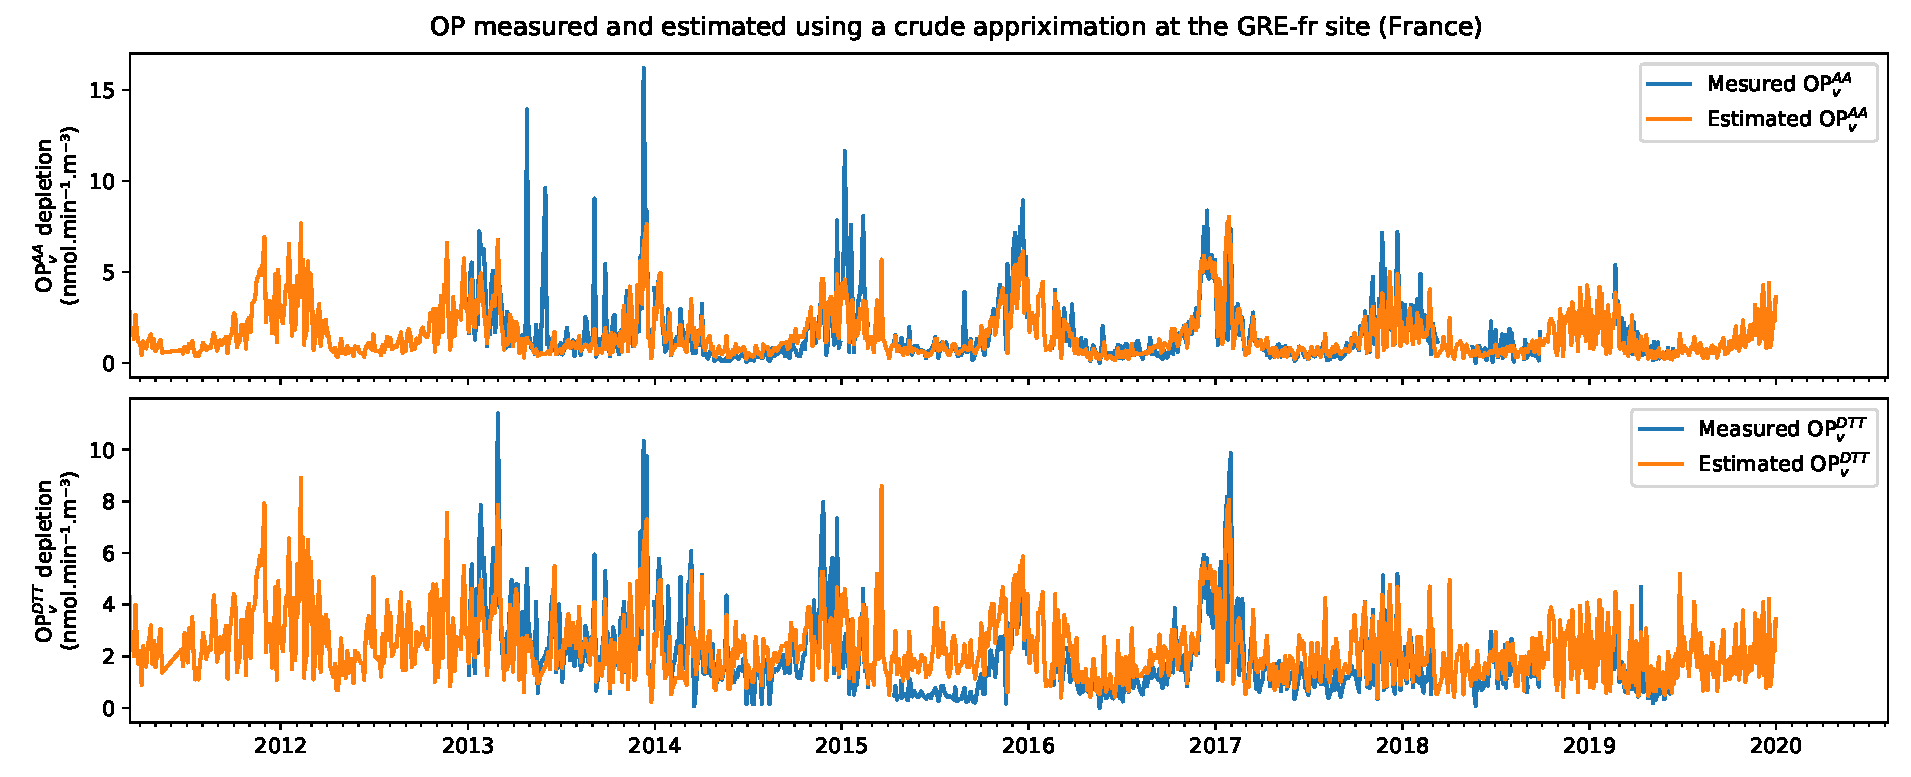
\includegraphics[width=1.0\textwidth]{figures/chapter05/OPGRE-fr_estimated.pdf}
    \caption{\POAAv{} (haut) et \PODTTv{} (bas) estimés en orange et mesurés en bleu sur le site de GRE-fr depuis 2011.}
    \label{fig:OPGRE-fr-estimated}
\end{figure}
 
\begin{figure}[ht]
    \centering
    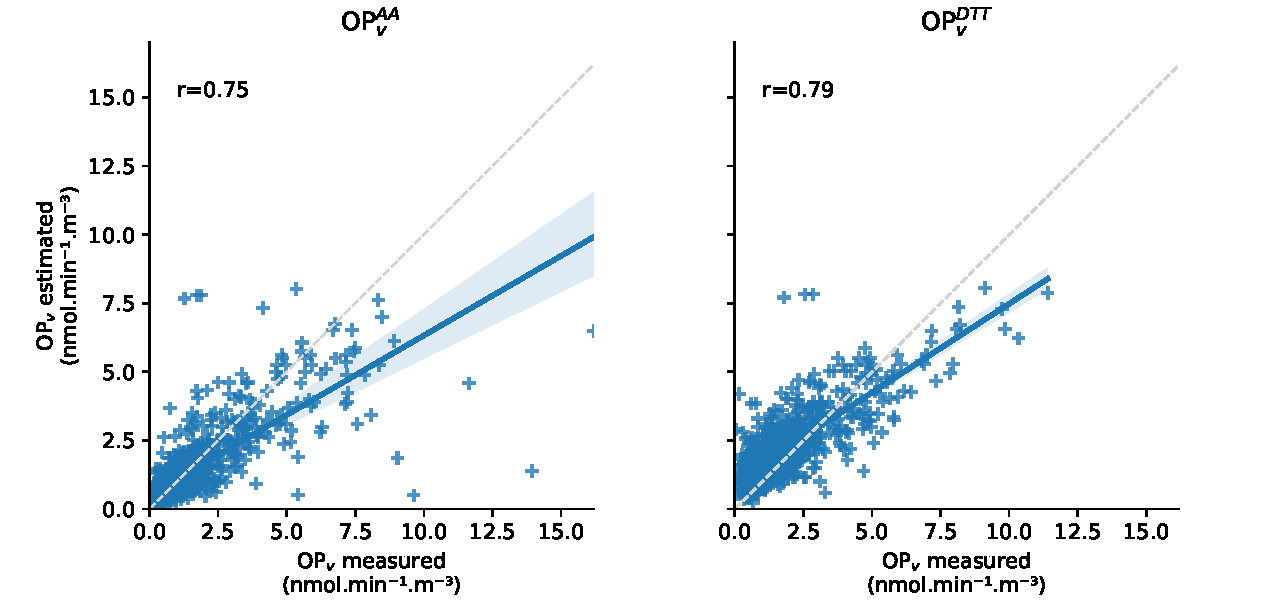
\includegraphics[width=0.8\textwidth]{figures/chapter05/OPGRE-fr_estimated_scatter.pdf}
    \caption{\POAAv{} et \PODTTv{} estimés et mesurés sur le site de GRE-fr depuis 2012.}
    \label{fig:OPGRE-fr-estimated_scatter}
\end{figure}


\begin{table}[ht]
    \centering
    \begin{tabular}{cccccccccc}
    Source & Aged_salt & Biomass_burning & Dust        & MSA_rich    & Nitrate_rich & Primary_biogenic & Road        & traffic     & Sulfate_rich\\
\multirow{7}{*}{DTTv}   & count     & 3162     & 3162 & 3162 & 3162  & 3162      & 3162 & 3162 & 3162\\
       & mean      & 0.070304        & 0.571739    & 0.392526    & 0.096813     & 0.131135         & 0.202920    & 0.668824    & 0.266885\\
       & std       & 0.036676        & 0.772676    & 0.214057    & 0.096970     & 0.142866         & 0.153622    & 0.395922    & 0.145060\\
       & min       & 0.003278        & 0.005868    & 0.016430    & 0.001685     & 0.004949         & 0.006725    & 0.057171    & 0.013217\\
       & 25\%      & 0.043976        & 0.043560    & 0.239088    & 0.027805     & 0.033403         & 0.084563    & 0.382064    & 0.162160\\
       & 50\%      & 0.064670        & 0.202108    & 0.361458    & 0.058053     & 0.073136         & 0.154738    & 0.568033    & 0.245227\\
       & 75\%      & 0.090800        & 0.829691    & 0.510741    & 0.140141     & 0.184638         & 0.286916    & 0.868082    & 0.348599\\
       & max       & 0.261221        & 4.162930    & 1.623681    & 0.772044     & 1.129129         & 0.937258    & 2.587625    & 1.170530\\
AAv    & count     & 3162     & 3162 & 3162 & 3162  & 3162      & 3162 & 3162 & 3162\\
       & mean      & 0.045093        & 0.871744    & 0.121530    & -0.014356    & 0.030154         & 0.051073    & 0.482702    & 0.031492\\
       & std       & 0.023524        & 1.178117    & 0.066274    & 0.014379     & 0.032852         & 0.038666    & 0.285744    & 0.017117\\
       & min       & 0.002103        & 0.008946    & 0.005087    & -0.114482    & 0.001138         & 0.001693    & 0.041261    & 0.001560\\
       & 25\%      & 0.028206        & 0.066417    & 0.074024    & -0.020781    & 0.007681         & 0.021284    & 0.275742    & 0.019135\\
       & 50\%      & 0.041479        & 0.308158    & 0.111911    & -0.008608    & 0.016818         & 0.038946    & 0.409959    & 0.028937\\
       & 75\%      & 0.058239        & 1.265049    & 0.158131    & -0.004123    & 0.042457         & 0.072215    & 0.626510    & 0.041134\\
       & max       & 0.167547        & 6.347317    & 0.502708    & -0.000250    & 0.259642         & 0.235901    & 1.867534    & 0.138121\\
    \end{tabular}
    \caption{Caption}
    \label{tab:my_label}
\end{table}V

\subsection{PO et CTM}
- Source dans les CTM (Chimère et LOTOS)
- Comparaison avec les PMF
- Inversion du PO par source CTM + Posttraitement avec PO / sources

\section{Non linéarité avec Réseaux de neurone}

\section{Exposition et épidémiologie}
\subsection{Mesure indoor et personnelle}
\subsection{Étude épidémio}

